\chapter{Propuesta de software}

Se desarrolló un programa capaz de brindar al usuario la posibilidad de realizar operaciones de inferencia causal. Las características que reúne el programa son las siguientes:
\begin{enumerate}
	\item Ofrecer una interfaz visual que permita a usuarios no expertos en programación realizar operaciones de inferencia causal. Dicha interfaz debe asistir al usuario tanto en la creación de los modelos como en las operaciones de inferencia causal, notificándolo en el caso de que existan errores en la entrada provista. 
	\item Permitir la construcción y visualización de SCMs. Debe permitir además exportar los modelos a ficheros externos para posteriormente ser cargados en el programa.
	\item Permitir realizar operaciones de inferencia causal sobre modelos causales estructurales. Ofrecer en un menú los distintos tipos de inferencia causal disponibles. Permitir al usuario seleccionar los parámetros que el programa tendrá en cuenta durante la inferencia.
	\item Ofrecer los resultados correspondientes a la consulta causal especificada por el usuario.
\end{enumerate}

\section{Implementación}		
El lenguaje de programación escogido para la implementación fue \textbf{Python} en su versión $3.8$. Su elección se debe a que es un lenguaje de alto nivel, multiparadigma  y con una filosofía que apuesta por un código legible y sencillo.

La implementación de la parte lógica del proyecto consiste de 3 módulos contenidos en un directorio llamado \textit{causality}. Estos módulos son:
\begin{itemize}
	\item \textit{main.py}: Contiene la implementación del SCM.
	\item \textit{tests.py}: Conjunto de tests unitarios destinados a probar las componentes fundamentales de la implementación.
	\item \text{util.py}: Conjunto de métodos auxiliares que serán utilizados desde otros módulos.
\end{itemize}

\subsection{Implementación del modelo causal estructural}
En el módulo \textit{main.py} se trabaja con un conjunto de clases para la implementación del modelo:	  

\begin{lstlisting}
	class Variable:
		def __init__(self, name, values):...
	
	class ExogenousVariable(Variable):
		def __init__(self, name, values, distribution):...
	
	class EndogenousVariable(Variable):
		def __init__(self, name, values, parents, expression):...
	
	class SCM:
		def __init__(self, exogenous_variables, endogenous_variables):...
\end{lstlisting}

La clase \textit{Variable} reúne las características comunes de las variables tanto exógenas como endógenas. Debe proveerse un nombre para la variable que la identifique en el modelo, por lo que este debe ser único. Además debe proveerse una lista de los valores que la variable puede tomar. La naturaleza de las variables es discreta y estas solo pueden tomar valores numéricos. Esta clase no se utiliza directamente sino que es heredada por las clases \textit{ExognousVariable} y \textit{EndogenousVariable}. 

La clase \textit{ExogenousVariable} representa a las variables exógenas de un SCM. Para crear una variable exógena se debe especificar su nombre, los valores que toma y su distribución de probabilidad. Dicha distribución consiste en una lista $P$ donde cada valor $P[i]$ se corresponde con la probabilidad de que la variable tome el valor $V[i]$, donde $V$ es la lista de valores provista. La lista debe cumplir con todas las propiedades de una distribución de probabilidad:
\begin{itemize}
	\item La suma de sus valores debe ser igual a 1
	\item Cada valor debe ser encontrarse en el intervalo $[0,1]$
\end{itemize}

En el caso de las variables endógenas, representadas por la clase \textit{EndogenousVariable} debe especificarse el nombre, los valores que toma, los padres de la variable (variables de las que depende) y la expresión que define a la misma. Es importante especificar todos los posibles valores que puede tomar la variable a partir de las variables de las que depende. Toda variable endógena debe depender de al menos otra variable y una de estas variables debe ser exógena. Esto último es necesario para el cálculo correcto de los contrafactuales, ya que el método utilizado (redes gemelas) utiliza las variables exógenas para conectar las variables del mundo real con las del mundo alternativo.

La expresión que define a la variable será una cadena con una sintaxis similar a las expresiones de Python. Además se podrán usar funciones de la clase \textit{math}, que viene integrada a dicho lenguaje. Ejemplo de posibles expresiones válidas son:
\begin{itemize}
	\item X + Y - 1
	\item (X and Y) if Z == 0 else (X or Y)
	\item max(X, Y) - min(X,Y)
\end{itemize}
Las variables que aparecen en las expresiones deben corresponderse con los nombres de las variables de las que depende la variable que se está definiendo.

Una vez creadas las variables exógenas y endógenas, estas se agrupan en dos listas y se llama al constructor de la clase $SCM$, la cual representa a los modelos causales estructurales.

Por ejemplo, si se tiene un modelo como el siguiente:

\begin{model}
	\label{model:sum}
	\[
	\arraycolsep=10pt
	\begin{array}{ccc}
		U = \{Ux, Uy, Uz\}&
		V = \{X, Y, Z\}&
		E = \{f_x, f_y, f_z\}
	\end{array}
	\]
	
	\[Val(Ux)=Val(Uy)=Val(X)=Val(Y)=\{0,1,2\}\]
	\[Val(Uz)=\{0, 1\}\]
	\[Val(Z)=\{0, 1, 2, 3, 4\}\]
	
	\begin{equation*}
		P(X=x)=  
		\left\{
		\begin{array}{ll}
			0.1 & \mathrm{si\ } x = 0\\
			0.2 & \mathrm{si\ } x = 1\\
			0.7 & \mathrm{si\ } x = 2\\
		\end{array}
		\right\}.
	\end{equation*}
	
	\begin{equation*}
		P(Y=y)=  
		\left\{
		\begin{array}{ll}
			0.2 & \mathrm{si\ } y = 0\\
			0.2 & \mathrm{si\ } y = 1\\
			0.6 & \mathrm{si\ } y = 2\\
		\end{array}
		\right\}.
	\end{equation*}
	
	\begin{equation*}
		P(Z=z)=  
		\left\{
		\begin{array}{ll}
			0.8 & \mathrm{si\ } z = 0\\
			0.2 & \mathrm{si\ } z = 1\\
		\end{array}
		\right\}.
	\end{equation*}
	
	\begin{center}
		\[
		\begin{array}{cc}
			f_x: & X = Ux\\
			f_y: & Y = Uy\\	
		\end{array}
		\]			
		\begin{equation*}
			f_z: Z=  
			\left\{
			\begin{array}{ll}
				X + Y & \mathrm{si\ } Uz = 0\\
				X * Y & \mathrm{si\ } Uz = 1\\
			\end{array}
			\right\}.
		\end{equation*}
	\end{center}
\end{model}

Entonces para construir dicho modelo se usaría el código:

\begin{lstlisting}
	Ux = ExogenousVariable("Ux", [0, 1, 2], [0.1, 0.2, 0.7])
	Uy = ExogenousVariable("Uy", [0, 1, 2], [0.2, 0.2, 0.6])
	Uz = ExogenousVariable("Uz", [0, 1], [0.8, 0.2])
	
	X = EndogenousVariable("X", [0, 1, 2], [Ux], "X")
	Y = EndogenousVariable("Y", [0, 1, 2], [Uy], "Y")
	Z = EndogenousVariable("Z", [0, 1, 2, 3, 4], [X, Y, Uz], "X + Y if Uz == 0 else X * Y")
	
	model = SCM([Ux, Uy, Uz], [X, Y, Z])
\end{lstlisting}

Los modelos también tienen una representación en formato JSON (Javascript Object Notation) con el objetivo de persisitirlos en ficheros y así poder usarlos posteriormente. El método \textit{export\_to\_json} convierte un objeto de tipo SCM a su representación en JSON, mientras que el método \textit{import\_from\_json} crea un objeto de tipo SCM a partir de la representación en JSON correspondiente. A su vez, los métodos \textit{export\_to\_json\_file} e \textit{import\_from\_json\_file} permiten guardar y cargar de memoria externa respectivamente.

\subsection{Algoritmos de inferencia}
La implementación de los algoritmos de inferencia causal se basa en la inferencia bayesiana. A la hora de responder a una pregunta causal se aplica un algoritmo que en algún punto pasa por la construcción de una red bayesiana y la ejecución de un algoritmo de inferencia para obtener la respuesta deseada.

Para el trabajo con redes bayesianas se utilizó la librería \textbf{pgmpy} \cite{ankan2015pgmpy}. Esta es una librería de código abierto para el trabajo con redes bayesianas, enfocada en la modularidad y la extensibilidad. Contiene implementaciones de algoritmos de estimación de parámetros, aprendizaje de estructura, inferencia exacta, aproximada y además inferencia causal.

El método \textit{build\_bayesian\_network} construye una red bayesiana a partir de un modelo causal estructural, mediante un proceso similar al descrito en la sección \ref{secc:scm-bn}. La parte más compleja de dicho algoritmo consiste en la creación de las tablas de probabilidad de las variables endógenas, donde es necesario computar todas las combinaciones posibles de valores que pueden tomar los padres más la variable. Así, si una variable $X$ depende de un conjunto $Pa_X=\{P_1, P_2, ..., P_n\}$ de variables, su tabla de probabilidad contaría con $|X| \cdot \prod_{i=1}^n |P_i|$ entradas, donde $|P_i|$ denota la cardinalidad de la variable $P_i$ y $|X|$ la cardinalidad de $X$. Para determinar el valor de cada probabilidad $P(X_i=x_i \mid Pa_X=x^{\ast})$ se evalúa la expresión que define a $X$ en la correspondiente asignación $x^{\ast}$ a las variables padres de $X$. Si el resultado es igual a $x_i$, entonces la probabilidad toma valor 1. En caso contrario toma valor 0. Para evaluar la expresión se utiliza la función \textit{eval} integrada a Python, que toma una expresión en forma de cadena de caracteres y los valores que se le asigna a las variables, y devuelve el resultado de evaluar dicha expresión.

Existen 3 tipos principales de inferencia en la implementación: predicciones, intervenciones y contrafactuales. Las signaturas de los métodos correspondientes a dichas operaciones se definen a continuación:

\begin{lstlisting}
	def predict(self, variables, observations={}, map=False, joint=False, algorithm="BP"):...
	
	def do_bayesian(self, variables, do_variables, observations={}, map=False, joint=False, algorithm="BP"):...
	
	def counterfactual(self, variables, do_variables, observations={}, map=False, joint=False, algorithm="BP"):...
\end{lstlisting}

El método \textit{predict} permite realizar una predicción en el modelo, devolviendo las probabilidades actualizadas de un conjunto de variables solicitadas (parámetro \textit{variables}) a partir de un conjunto de variables observadas (\textit{observations}). Por ejemplo, si se quiere determinar la probabilidad $P(Y \mid X=1)$ se hece la llamada siguiente al método:	
\begin{lstlisting}
	result = model.predict(["Y"], observations={"X": 1})
\end{lstlisting}	
El método \textit{do\_bayesian} calcula el resultado de una intervención, incorporando el parámetro \textit{do\_variables} que indica las variables que son intervenidas y los valores que son forzados a tomar. Suponiendo que se quiere calcular $P(Y \mid do(X=1), Z=2)$ la llamada al método sería:
\begin{lstlisting}
	result = model.do_bayesian(["Y"], {"X": 1}, observations={"Z": 2})
\end{lstlisting}

Para calcular el resultado de la intervención se usa el procedimiento descrito en la sección \ref{sec:do-bn}: se construye el submodelo correspondiente a la intervención mediante el método \textit{get\_submodel}, y convirtiéndolo en red bayesiana con el método \textit{build\_bayesian\_network} se aplica inferencia para obtener la respuesta deseada. 

El método \textit{counterfactual} calcula el resultado de un contrafactual, recibiendo los mismos parámetros que el método \textit{do\_bayesian} pero con un significado ligeramente distinto: las variables de la respuesta deben corresponder al mundo alternativo, para lo cual se debe añadir el caracter \textquoteleft*\textquoteright al final del nombre de la variable, y lo mismo ocurre con las variables especificadas en \textit{do\_variables} que corresponden a las intervenciones realizadas en el mundo alternativo. Para calcular el contrafactual $P(Y_{X=1} \mid Z=z)$ la llamada al método \textit{counterfactual} sería:
\begin{lstlisting}
	result = model.counterfactual(["Y*"], {"X*": 1},observations={"Z": 2})
\end{lstlisting}
Para calcular el contrafactual se utiliza el método de las redes gemelas descrito en la sección \ref{sec:tn}. Se construye la estructura mediante el método \textit{build\_twin\_network} que a partir de un modelo construye el modelo de redes gemelas correspondiente. La respuesta al contrafactual se obtiene llamando al método \textit{do\_bayesian} sobre el modelo de redes gemelas resultante.

Los métodos anteriores disponen de un conjunto de parámetros opcionales . El parámetro \textit{map} especifica si en vez de realizar inferencia probabiliística se debe realizar inferencia MAP. El parámetro \textit{joint} indica si se desea obtener en la respuesta la distribución de probabilidad conjunta o las distribuciones por separado. El parámetro \textit{algorithm} indica el algoritmo de inferencia que será usado y puede tomar dos valores: \textquotedblleft BP \textquotedblright(propagación de creencias) y \textquotedblleft VE\textquotedblright(eliminación de variables).	

En caso de que la inferencia especificada sea probabilística, los métodos \textit{predict}, \textit{do\_bayesian} y \textit{counterfactual} devuelven una función. Si es solicitada la distribución conjunta, esta recibe como parámetro una asignación en forma de diccionario de los valores que toma cada variable y devuelve la probabilidad correspondiente. Si no se pide la distribución conjunta, entonces la función devuelta recibe como parámetro el nombre de una variable de la respuesta y el valor que toma, devolviendo la probabilidad correspondiente. Por otro lado, si se especifica que la inferencia es de tipo MAP, entonces se devuelve un diccionario con la asignación más probable a las variables.

Por ejemplo, para el modelo \ref{model:sum}, si deseamos obtener el valor de $P(Z_{X=1}=3 | Z=3)$, la instrucción de código quedaría:
\begin{lstlisting}
	model.counterfactual(["Z*"], {"X*": 1}, {"Z": 3})("Z*", 3)
\end{lstlisting}
En cambio la probabilidad conjunta $P(Z=3, Y=2 | do(X=1))$ se obtendría así:
\begin{lstlisting}
	model.do_bayesian(["Z", "Y"], {"X": 1})({"Z": 3, "Y": 2})
\end{lstlisting}
Por otro lado la asignación más probable MAP($Z, Y | do(X=1)$) se obtendría leyendo el diccionario que devuelve el llamado al método \textit{do\_bayesian\_map}:
\begin{lstlisting}
	result = model.do_bayesian(["Y", "Z"], {"X": 1}, map=True)
	for variable, value in result.items():
		print(variable, value)
\end{lstlisting}

Como se vio en las secciones \ref{sec:attr} y \ref{sec:med}, las fórmulas de mediación y atribución se definen en términos de intervenciones y contrafactuales y por tanto su implementación es inmediata. En el caso de la atribución se reciben dos parámetros correspondientes al tratamiento(causa) y la respuesta(efecto). Cada uno de estos parámetros consiste en una tupla de tres elementos de la forma (nombre de la variable, valor verdadero, valor falso):

\begin{lstlisting}
	def prob_of_neccesity(self, cause, effect):...
	
	def prob_of_sufficiency(self, cause, effect):...
	
	def prob_of_neccesity_and_sufficiency(self, cause, effect):...
\end{lstlisting}

Por ejemplo si se tienen dos variables binarias $X$, $Y$, y se quiere calcular la necesidad de tomar un medicamento($X=1$) para recuperarse ($Y=1$), entonces el llamado al método \textit{prob\_of\_neccesity} sería:

\begin{lstlisting}
	model.prob_of_neccesity(self, ("X", 1, 0), ("Y", 1, 0))
\end{lstlisting}

Las fórmulas de mediación implementadas son el efecto total y el efecto directo controlado, que aplican para dos pares de variables cualesquiera:

\begin{lstlisting}
	def total_effect(self, cause, effect_variable):...
	
	def controlled_direct_effect(self, cause, effect_variable, mediator):...
\end{lstlisting}

Ambas reciben un parámetro \textit{cause} que consiste en una tupla (nombre de la causa, valor inicial, valor final) y otro parámetro \textit{effect\_variable} que indica el nombre de la variable en la que se mide el efecto. Si quisiésemos medir el efecto total de $X$ en $Y$ cuando $X$ cambia de $0$ a $1$, entonces llamaríamos a la primera función con los parámteros:
\begin{lstlisting}
	model.total_effect(("X", 0, 1), "Y")
\end{lstlisting}

El efecto directo controlado recibe otro parámetro que consiste en una tupla (nombre, valor) correspondiente al mediador que se está analizando. Una posible llamada al método sería:
\begin{lstlisting}
	model.controlled_direct_effect(("X", 0, 1), "Y", ("Z", 0))
\end{lstlisting}
Aquí se calcula el efecto de $X$ en $Y$ cuando el mediador $Z$ es obligado a tomar el valor $0$.

\subsection{Complejidad}
La complejidad de los algoritmos de inferencia causal es exponencial ya que todos utilizan un algoritmo de inferencia bayesiana exacta que puede ser propagación de creencias \cite{lauritzen1988local}, cuya complejidad es exponencial con respecto al tamaño del mayor clique del grafo moral triangulado, o eliminación de variables \cite{zhang1994simple}, cuya solución pasa por encontrar un conjunto de variables de eliminación óptimo, siendo este un problema NP-completo.

\begin{dfn}
	Sea $G = \langle V, E \rangle$ un grafo dirigido donde $N = |V|$ y $M = |E|$. El coeficiente de densidad de $G$ es:
	\[D_G = \frac{M}{N^2}\]
\end{dfn}

\begin{dfn}
	Un grafo $G$ es esparcido si $D_G \le 0.08$. En caso contrario se dice que es denso.
\end{dfn}

El tiempo de ejecución de los algoritmos depende de varios factores: el número de nodos o tamaño del grafo, la densidad del grafo y la cantidad máxima de valores que puede tomar cada variable. Se obtuvieron resultados satisfactorios para grafos esparcidos y con variables que toman un número pequeño de valores.

Los tiempos de ejecución obtenidos para las predicciones fueron muy similares a los de las intervenciones. Esto tiene sentido, puesto que una predicción es una intervención sobre un conjunto vacío de variables. 

En las predicciones se comportó ligeramente mejor el algoritmo de propagación de creencias que el de eliminación de variables. La Figura \ref{fig:p-24} compara el comportamiento de los dos, tiendo en cuenta distintas cardinalidades máximas para las variables del modelo (valor de $v$).  La Figura \ref{fig:p-bp-8-60} muestra el comportamiento de las predicciones usando el algoritmo de propagación de creencias en modelos de hasta 60 variables donde todas son binarias.

\begin{figure}[h!]
	\centering
	\begin{subfigure}{.49\linewidth}
		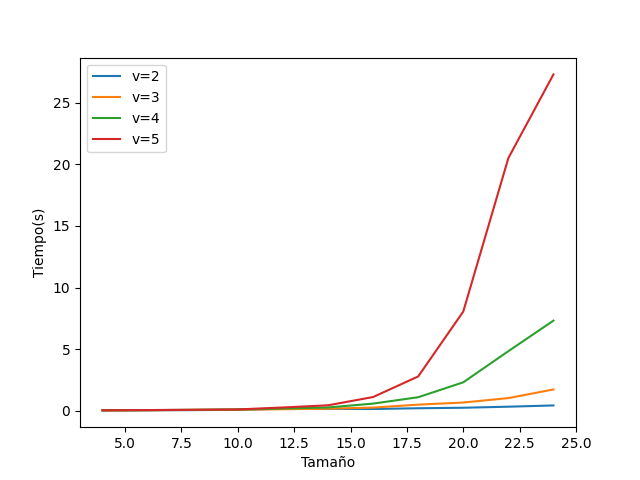
\includegraphics[width=\linewidth]{./images/Chapter-3/p-bp-8-24}
		\caption{BP}
	\end{subfigure}
	\begin{subfigure}{.49\linewidth}
		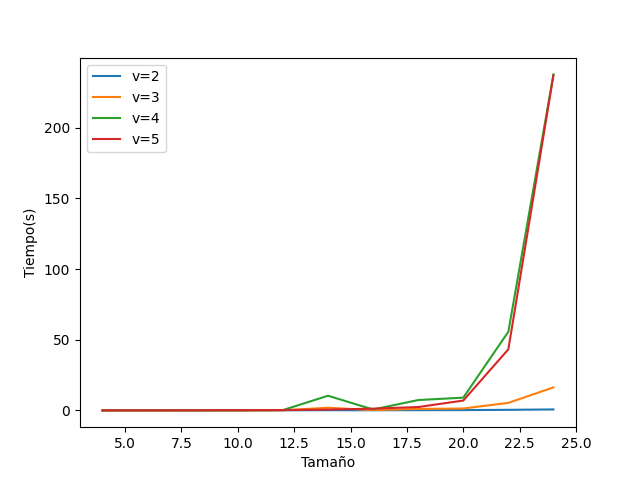
\includegraphics[width=\linewidth]{./images/Chapter-3/p-ve-8-24}
		\caption{VE}
	\end{subfigure}
	\caption{Comparación entre los algoritmos de propagación de creencias y eliminación de variables}
	\label{fig:p-24}
\end{figure}

\begin{figure}[h!]
	\centering
	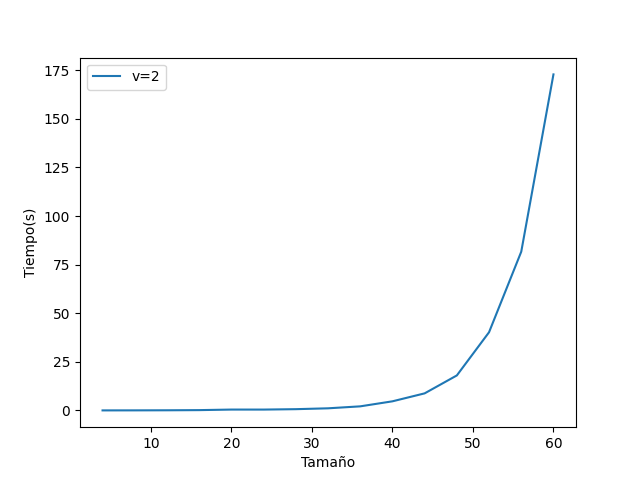
\includegraphics[width=0.5\linewidth]{./images/Chapter-3/p-bp-8-60}
	\caption{Comportamiento del algoritmo de propagación de creencias para modelos con sólo variables binarias}
	\label{fig:p-bp-8-60}
\end{figure}

Los contrafactuales resultaron ser viables en redes más pequeñas que las de las predicciones e intervenciones, pues el método de las redes gemelas transforma la red en una de casi el doble de su tamaño y realiza inferencia sobre ella. En la Figura \ref{fig:c-8-20} se muestra el comportamiento de los contrafactuales en dependencia del algoritmo que se use durante la fase de inferencia bayesiana en modelos con solo variables binarias.

\begin{figure}[h!]
	\centering
	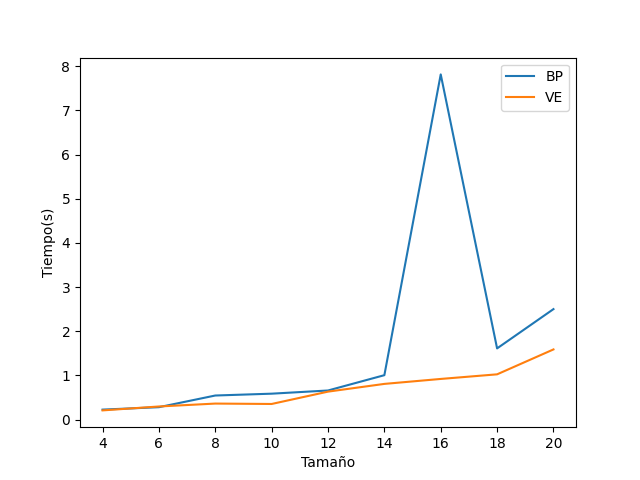
\includegraphics[width=0.5\linewidth]{./images/Chapter-3/c-8-20}
	\caption{propagación de creencias vs eliminación de variables en contrafactuales}
	\label{fig:c-8-20}
\end{figure}




\section{Interfaz de usuario}
La interfaz de usuario está concebida para facilitar el uso de la inferencia causal en problemas que lo requieran, abstrayendo al usuario del ambiente de la programación. Se brinda al usuario la posibilidad de crear, editar, cargar y guardar modelos estructurales causales. Además es posible visualizar el grafo causal asociado. Se brindan 5 modalidades de inferencia causal: predicción, intervención, contrafactual, atribución y mediación. Para cada tipo de inferencia se provee un formulario donde el usuario especifica los parámetros de la consulta a realizar. Para asegurar que la entrada provista por los usuarios al programa es la correcta, en todos los formularios existen métodos de validación que notifican al usuario en caso de que la entrada sea incorrecta.

La interfaz visual fue desarrollada con la librería \textbf{kivy}\cite{kivyDocs}. Entre sus principales características se encuentran que es de código abierto, multiplataforma y eficiente. Permite la creación de aplicaciones de manera rápida y a diferencia de otras librerías para interfaces visuales como PyQt, ofrece una sintaxis más elegante, al estilo de Python.

Para la visualización de los grafos causales se utilizaron dos librerías: \textbf{pydot}\cite{pydotDocs} y \textbf{networkx}\cite{networkxDocs}. Ello se debe a que en algunas arquitecturas de sistemas operativos la primera, que es la preferida, requiere de la instalación de dependencias adicionales, y no se desea que esa tarea recaiga en manos del usuario. Por ello cuando se solicita la imagen de un grafo causal, se da prioridad a \textit{pydot}, y en caso de que no sea posible utilizarla, se usa la segunda, que es más flexible.

Por último, para el proceso de empaquetado del software se utilizó \textbf{PyInstaller}\cite{PyInstaller}. Esta librería agrupa el código y las dependencias en un paquete que puede ser usado en otras computadoras sin la necesidad de instalar un intérprete de Python ni las dependencias, siempre y cuando sea en un sistema operativo similar a donde se construyo el paquete.

\begin{figure}
	\centering
	\begin{subfigure}{\linewidth}
		\centering
		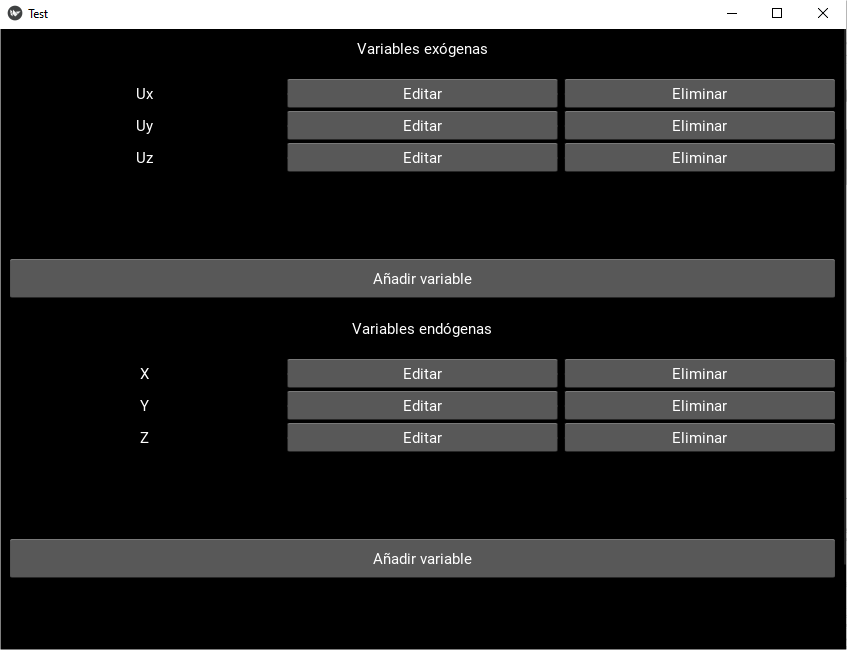
\includegraphics[width=300px, height=280px]{./images/Chapter-3/create-model}
		\caption{Ventana de creación de un modelo causal estructural}
		\label{fig:create-model}
	\end{subfigure}
	\begin{subfigure}{\linewidth}
		\centering
		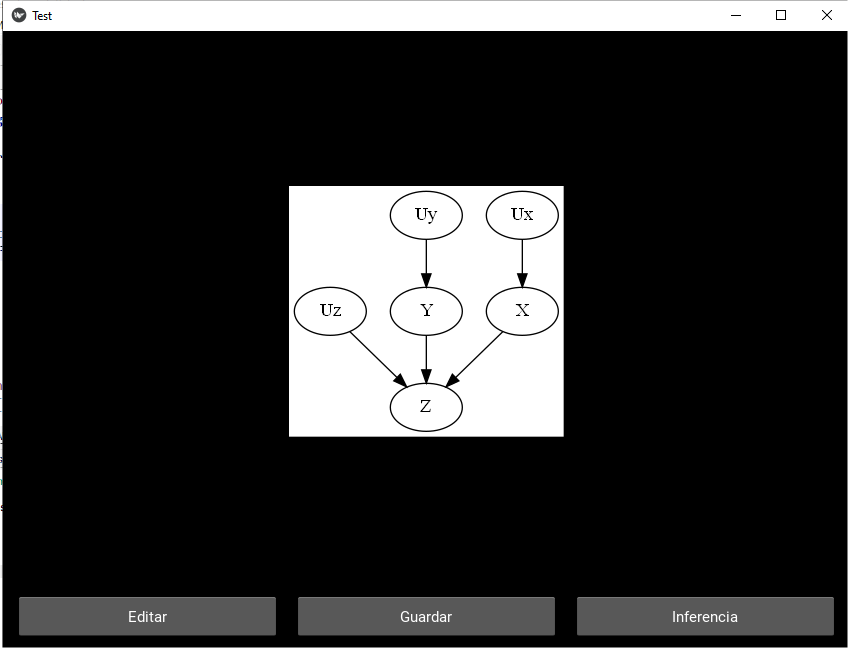
\includegraphics[width=300px, height=280px]{./images/Chapter-3/model-view}
		\caption{Ventana principal del modelo}
		\label{fig:model-view}
	\end{subfigure}
\end{figure}

\begin{figure}
	\begin{subfigure}{\linewidth}
		\centering
		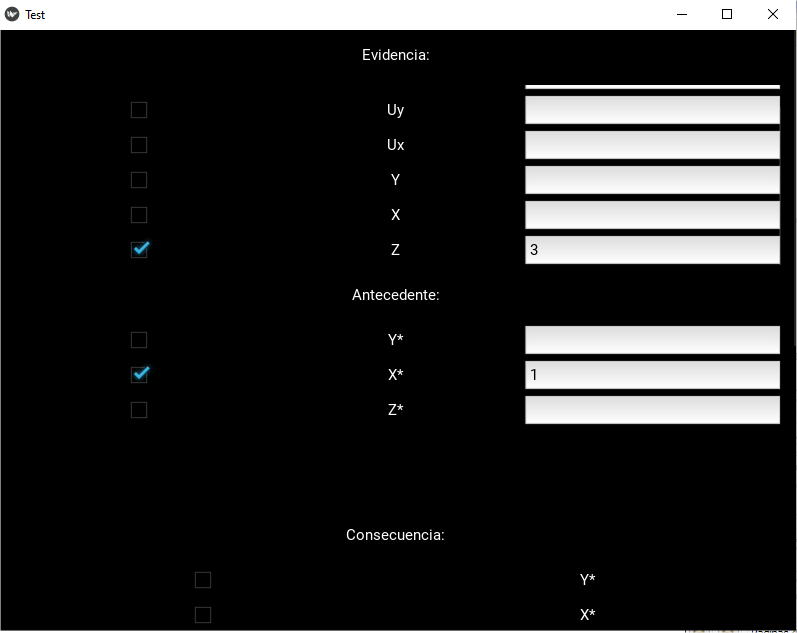
\includegraphics[width=300px, height=280px]{./images/Chapter-3/counterfactual(1)}
		\subcaption{}
		\label{fig:counterfactual-1}
	\end{subfigure}
	\begin{subfigure}{\linewidth}
		\centering
		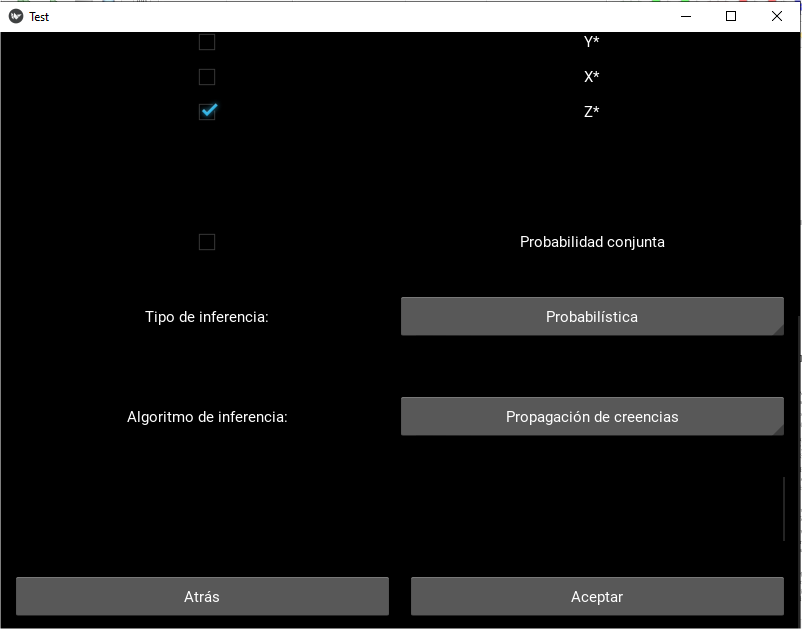
\includegraphics[width=300px, height=280px]{./images/Chapter-3/counterfactual(2)}
		\subcaption{}
		\label{fig:counterfactual-2}
	\end{subfigure}
	\subcaption{Formulario para calcular un contrafactual}
	\label{fig:counterfactual}
\end{figure}

\begin{figure}
	\centering
	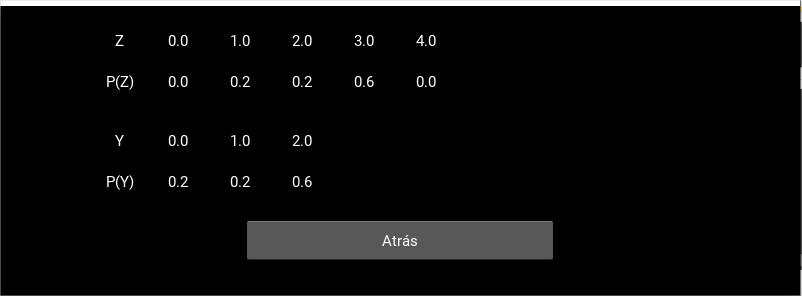
\includegraphics[width=300px, height=280px]{./images/Chapter-3/intervention-result}
	\caption{Resultados de una intervención}
	\label{fig:intervention}
\end{figure}